\section{Общие сведения теории формальных языков}

В данной главе мы рассмотрим основные понятия из теории формальных языков, которые пригодятся нам в дальнейшем изложении.

\begin{definition}
\textit{Алфавит} --- это конечное множество.
Элементы этого множества будем называть \textit{символами}.
\end{definition}

Традиционное обозначение для алфавита --- $\Sigma$.
Также мы будем использовать различные прописные буквы латинского алфавита.

Будем считать, что над алфавитом $\Sigma$ всегда определена операция конкатенации $(\cdot): \Sigma^* \times \Sigma^* \to \Sigma^*$.
При записи выражений символ точки (обозначение операции конкатенации) часто будем опускать: $a \cdot b = ab$.

\begin{definition}
\textit{Слово} над алфавитом $\Sigma$ --- это конечная конкатенация символов алфавита $\Sigma$: $\omega = a_0 \cdot a_1 \cdot \ldots \cdot a_m$, где $\omega$ --- слово, а для любого $i$ $a_i \in \Sigma$.
\end{definition}

\begin{definition}
\textit{Слово} над алфавитом $\Sigma$ --- это результат конечной конкатенации символов алфавита $\Sigma$: $\omega = a_0 \cdot a_1 \cdot \ldots \cdot a_m$, где $\omega$ --- слово, а для любого $i$ $a_i \in \Sigma$.
Будем называть $m + 1$ длиной слова и обозначать как $|\omega|$.
\end{definition}

\begin{definition}
\textit{Язык} над алфавитом $\Sigma$ --- это множество слов над алфавитом $\Sigma$.
\end{definition}

Заметим, что язык не обязан быть конечным множеством, в то время как алфавит обязан быть конечным и изучаем мы конечные слова.

\begin{definition}
\textit{Способы задания языков}
\begin{itemize}
\item Перечислить для онечных
\item Генератор
\item Распознователь
\end{itemize}

\end{definition}

\subsection{Контекстно-свободные грамматики и языки}

Из всего многообразия нас будут интересовать прежде всего контекстно-свободные грамматики.

\begin{definition}
\textit{Контекстно-свободная грамматика} --- это четвёрка вида $\langle \Sigma, N, P, S \rangle$, где
\begin{itemize}
  \item $\Sigma$ --- это терминальный алфавит;
  \item $N$ --- это нетерминальный алфавит;
  \item $P$ --- это множество правил или продукций, таких что кажая продукция имеет вид $N_i \to \alpha$, где $N_i \in N$ и $\alpha \in \{\Sigma \cup N\}^* \cup {\varepsilon}$;
  \item $S$ --- стартовый нетерминал.
  Отметим, что $\Sigma \cap N = \varnothing$.
\end{itemize}
\end{definition}

\begin{definition}
\textit{Отношение выводимости}
\end{definition}

\begin{definition}
\textit{Вывод слова в граммтике}
\end{definition}

\begin{definition}
\textit{Левосторонний вывод}
\end{definition}

Аналогично можно определить правосторонний вывод.

\begin{definition}
\textit{Язык, задаваемый граммтикой}
\end{definition}

Неоднозначные граммтики.

Существенно неоднозначные языки.


\subsection{Дерево вывода}
В некоторых случаях не достаточно знать порядок рименения правил.
Необходимо структурное представление вывода цепочки в граммтике.
Таким представлением является \textit{дерево вывода}.
\begin{definition}
Деревом вывода цепочки $\omega$ в граммтике $G=\langle \Sigma, N, S, P \rangle$ называется дерево, удовлетворяющее следующим свойствам.

\begin{enumerate}
  \item Помеченное: метка каждого внутреннего узла --- нетерминал, метка каждого листа --- терминал или $\varepsilon$.
  \item Корневое. Корень помечен стартовым нетерминалом.
  \item Упорядоченное.
  \item В дереве есть узел с меткой $N_i$ и сыновьями $M_j \dots M_k$ тогда и только тогда, когда в грамматике есть правило вида $N_i \to M_j M_k$.
  \item Крона --- цепочка.
\end{enumerate}
\end{definition}

\begin{example}
  Построим дерево вывода цепочки $ababab$ в граммтике $G = \langle \{a,b\}, \{S\}, S, {S \to a \ S \ b \ S, S \to \varepsilon} \rangle$.

  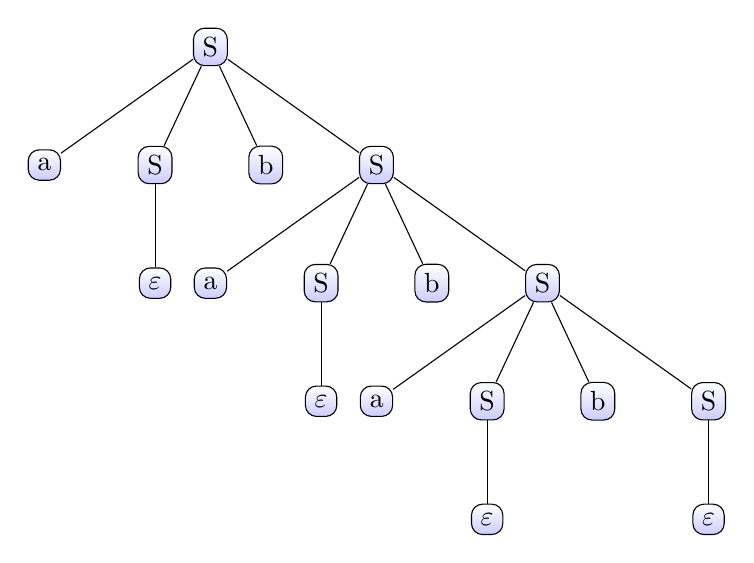
\begin{tikzpicture}[sibling distance=4em,
  every node/.style = {shape=rectangle, rounded corners,
    draw, align=center,
    top color=white, bottom color=blue!20}]]
  \node {S}
    child { node {a} }
    child { node {S}
      child { node {$\varepsilon$}}
    }
    child { node {b} }
    child { node {S}
      child {node {a}}
      child { node {S}
        child { node {$\varepsilon$}}
      }
      child { node {b} }
      child { node {S}
        child {node {a}}
        child {node {S}
          child {node {$\varepsilon$}}
        }
        child {node {b}}
        child {node {S}
          child {node {$\varepsilon$}}
        }
      }
    };
\end{tikzpicture}

\end{example}


\subsection{Нормальная форма Хомского}
\label{section:CNF}

\begin{definition}
Определение НФХ.
\end{definition}

\begin{theorem}
Любую КС граммтику можно преобразовать в НФХ.
\end{theorem}


\subsection{Вопросы и задачи}
\begin{enumerate}
  \item Предъявить несколько выовдов для одной цепочки.
  \item Построить выводы
  \item Построить деревья вывода !!! Перенести из раздела про SPPF
\end{enumerate}
